\section{Results}
\label{sec:results}

We have implemented and tested four of our methods on several synthetic datasets.
Each synthetic dataset embeds a low-dimensional manifold in high-dimensional space.
In each dataset, approximately $5\%$ of the points are random noise, i.e. outliers.
We examine the effectiveness our methods by their ability to find these outliers.

Figure~\ref{results:datasets} shows the ``Bullseye'' data and the ``Spiral'' data in 2-space, and the ``Interlocking Tori'' data and the ``Skewer'' data in 3-space.
We chose to test on non-linear manifolds because detecting anomalies on linear manifolds is fairly simple.

\begin{figure}[!t]
\centering
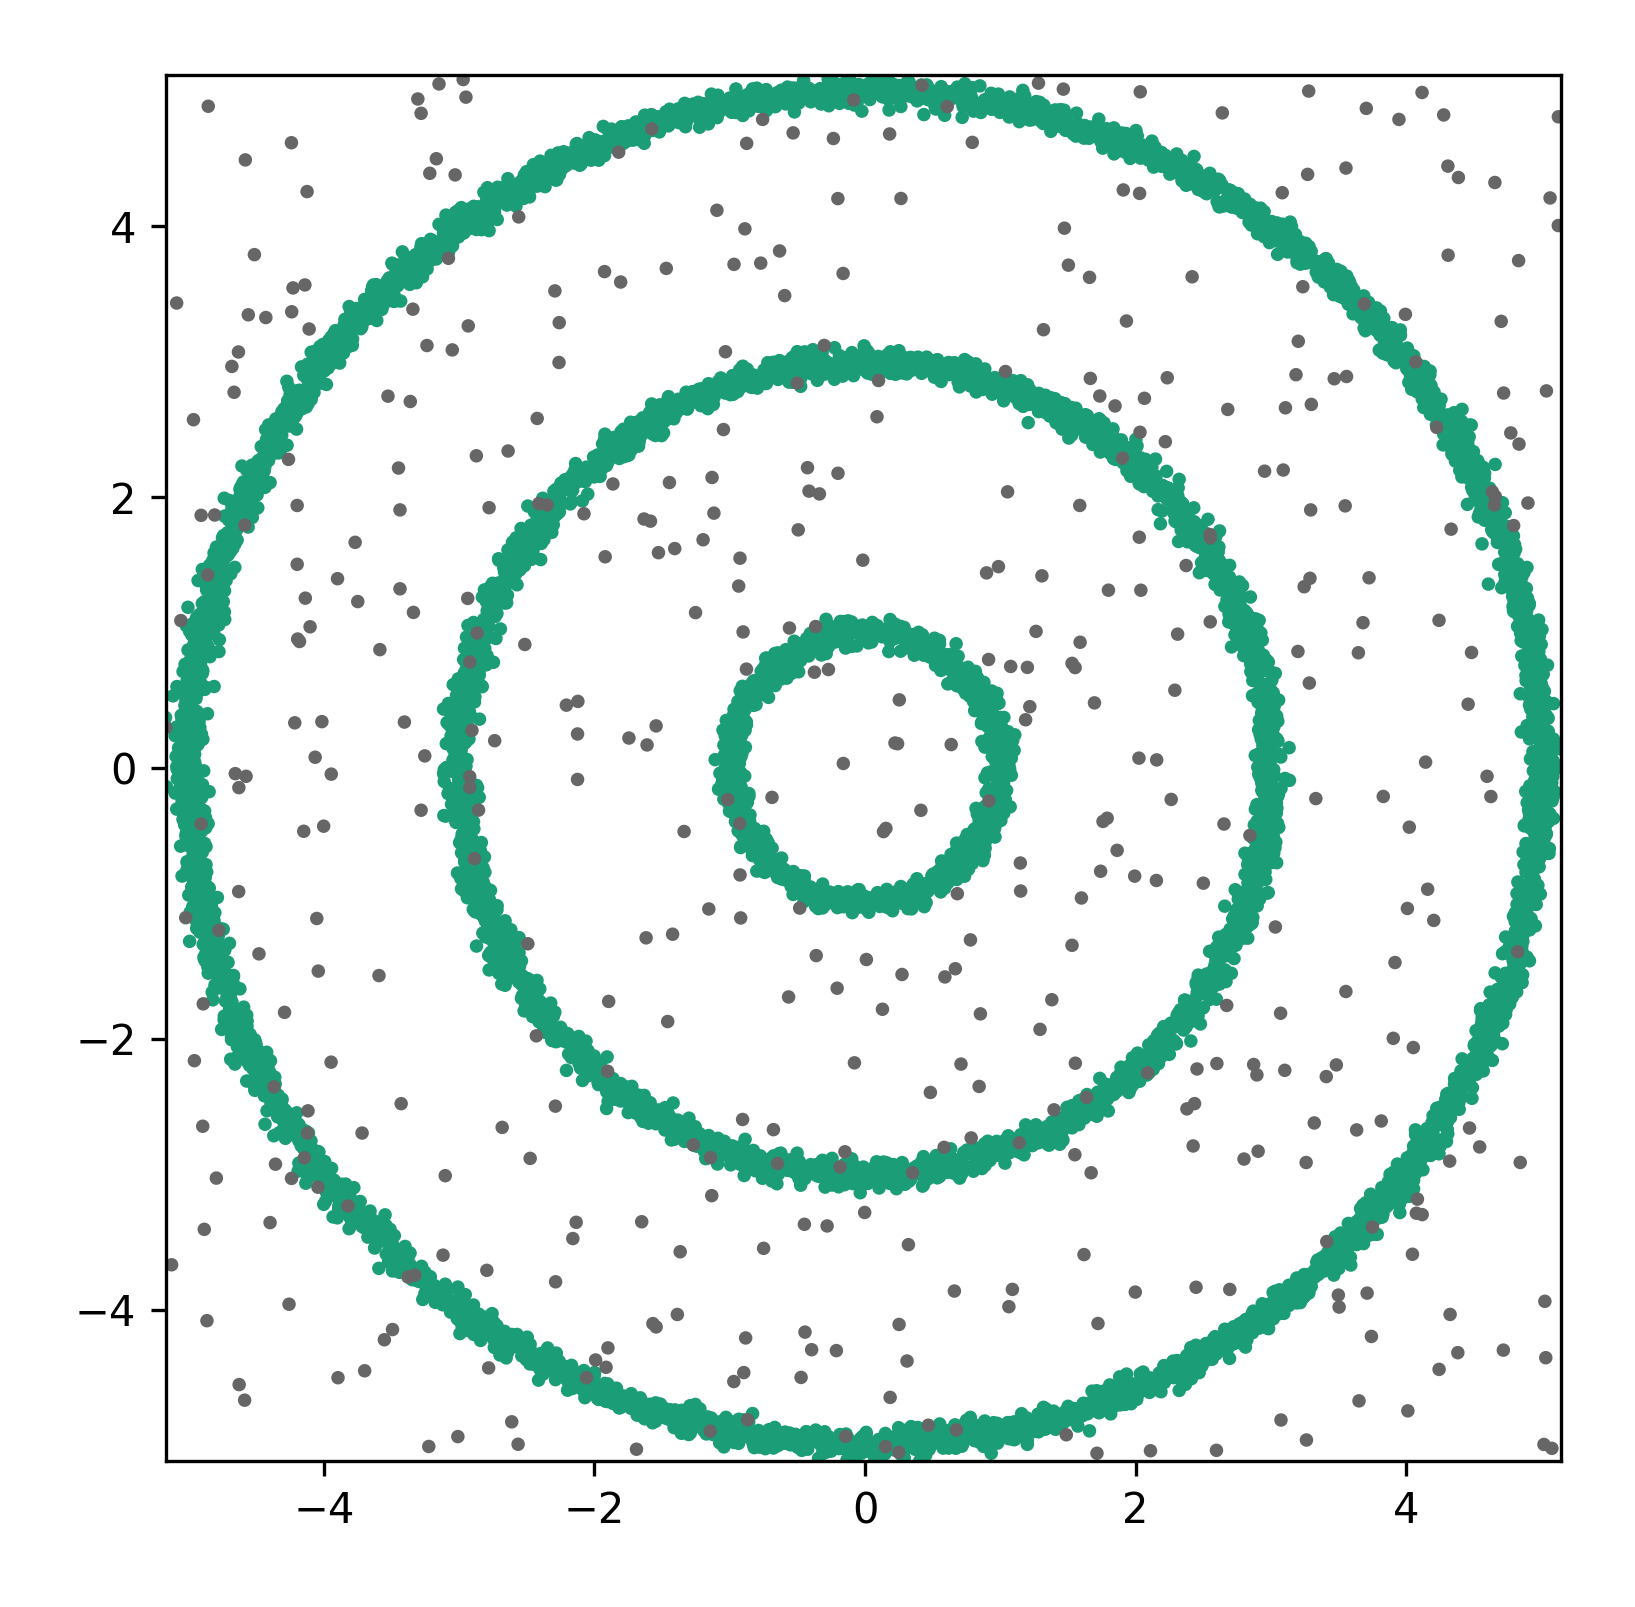
\includegraphics[width=2.5in]{static/bullseye.png}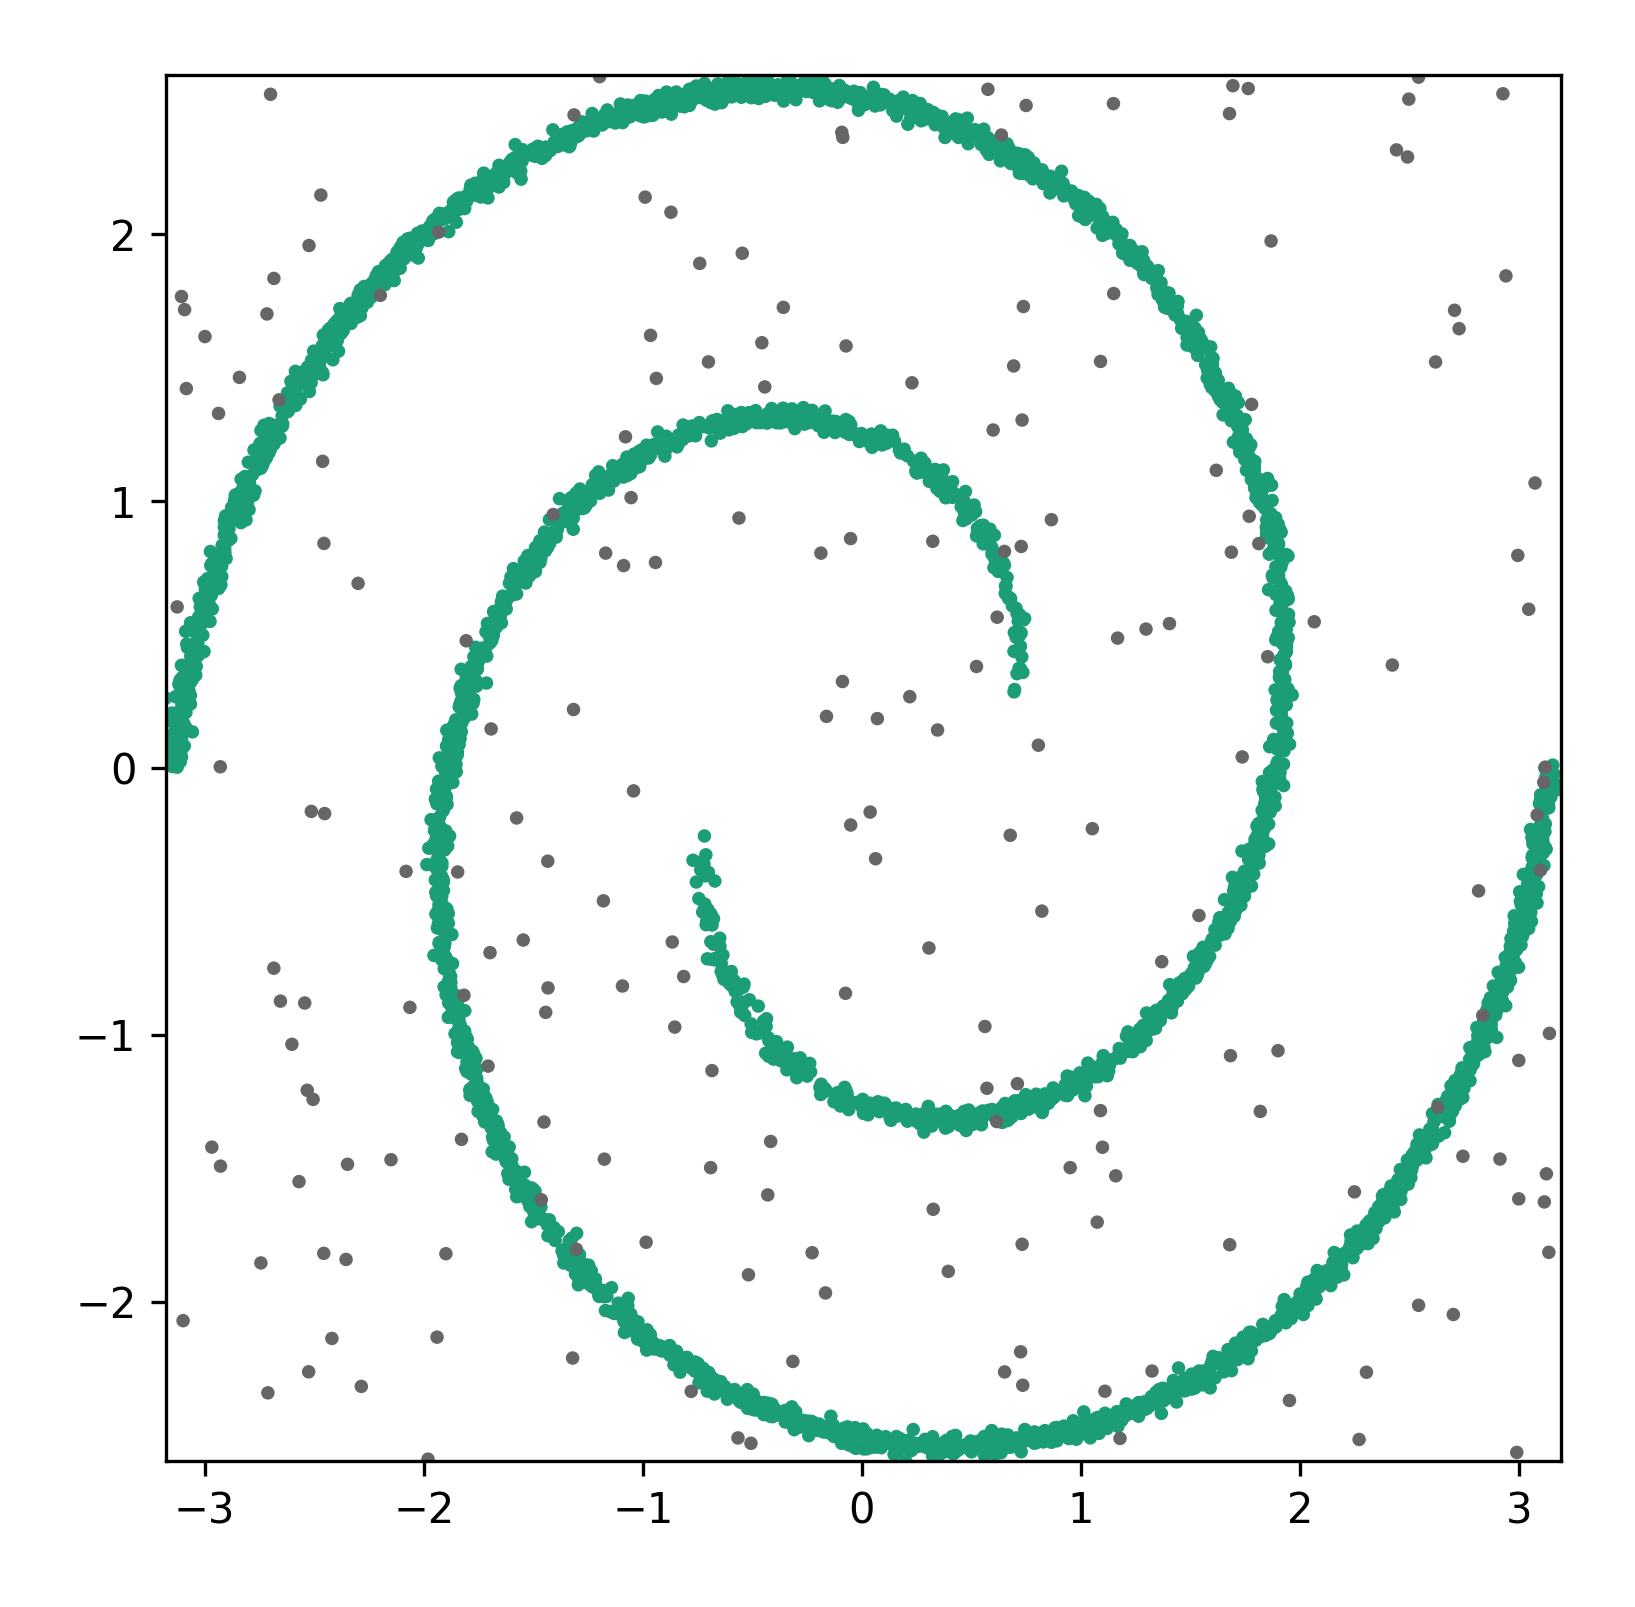
\includegraphics[width=2.5in]{static/spiral.png}

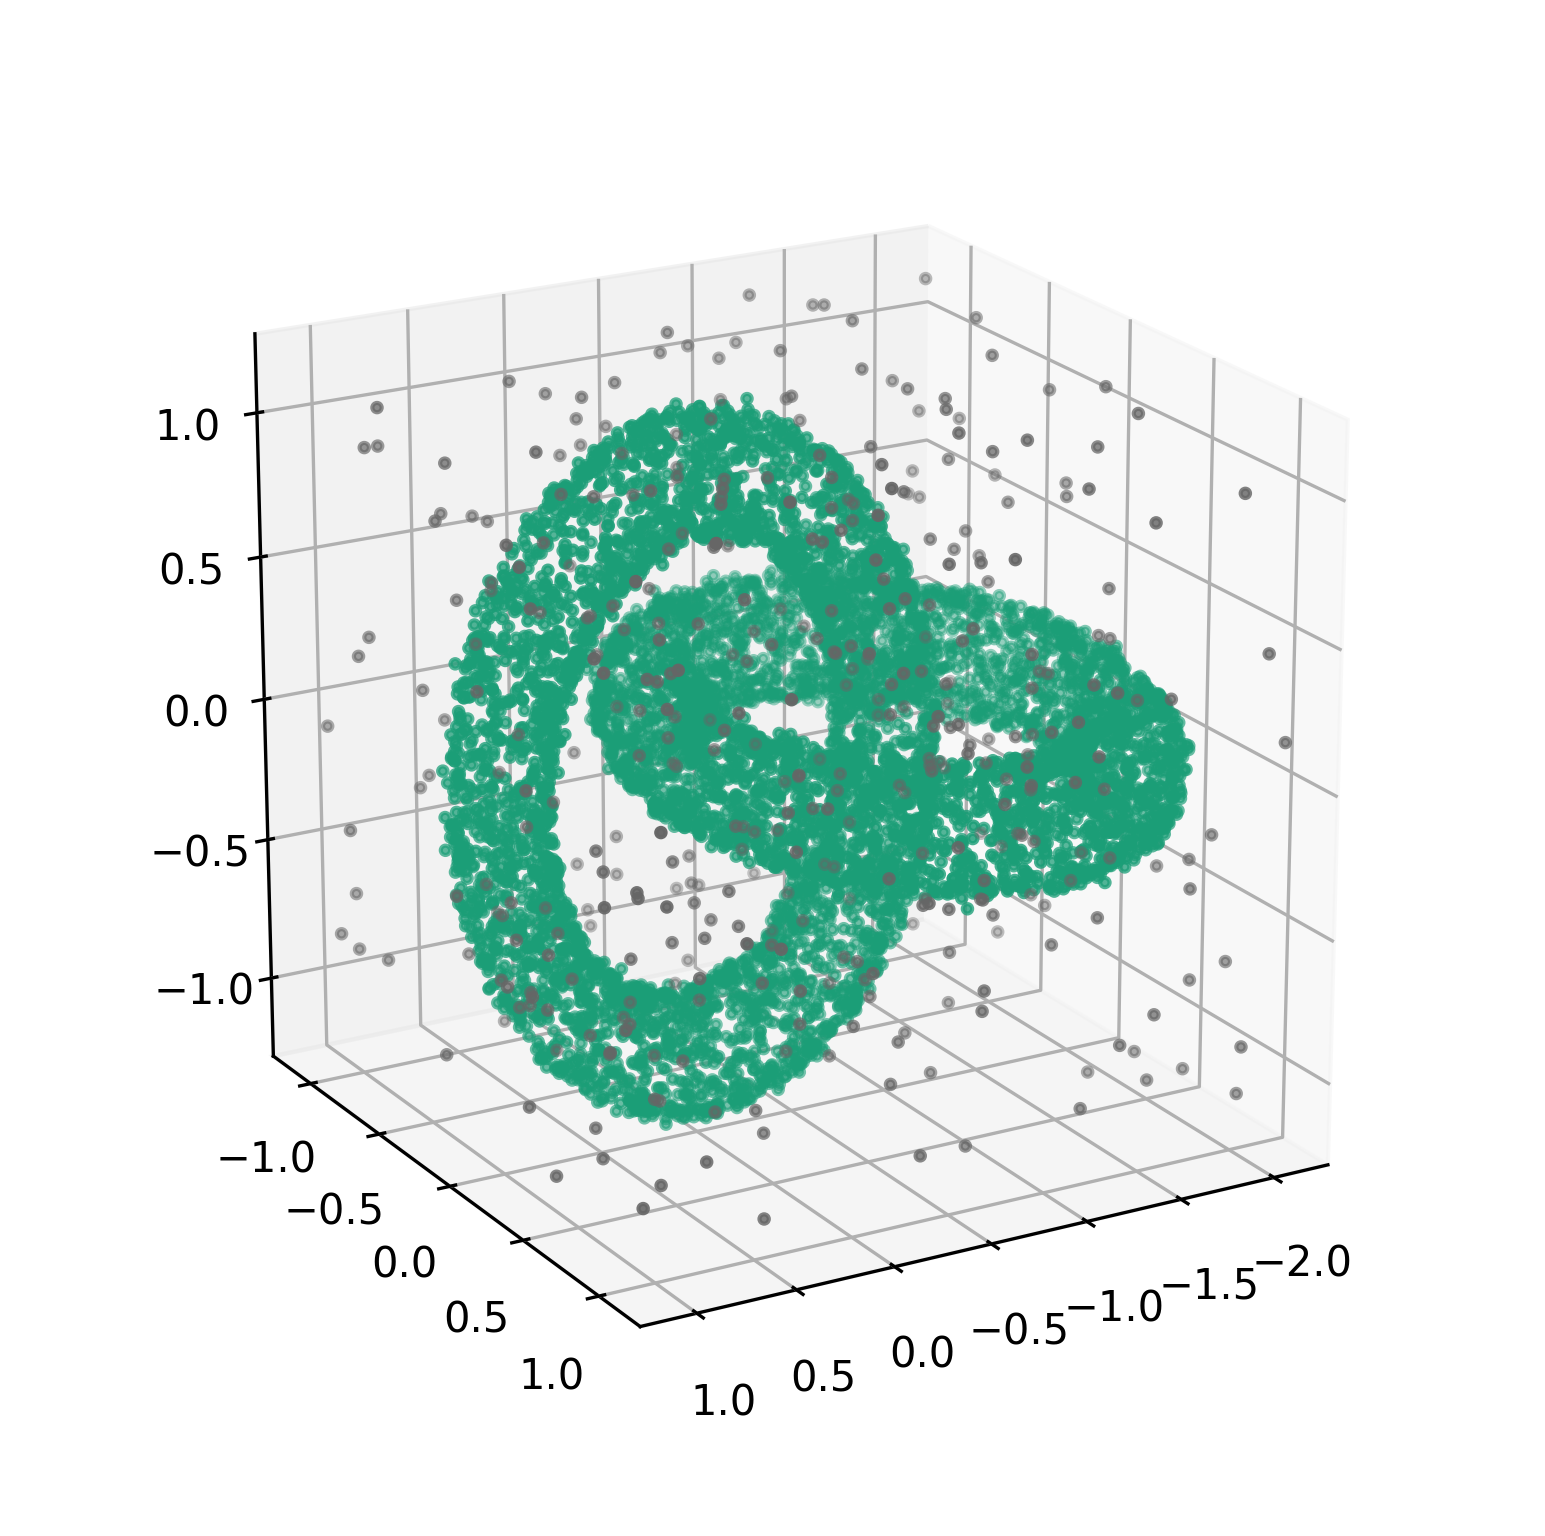
\includegraphics[width=3in]{static/interlocking_tori.png}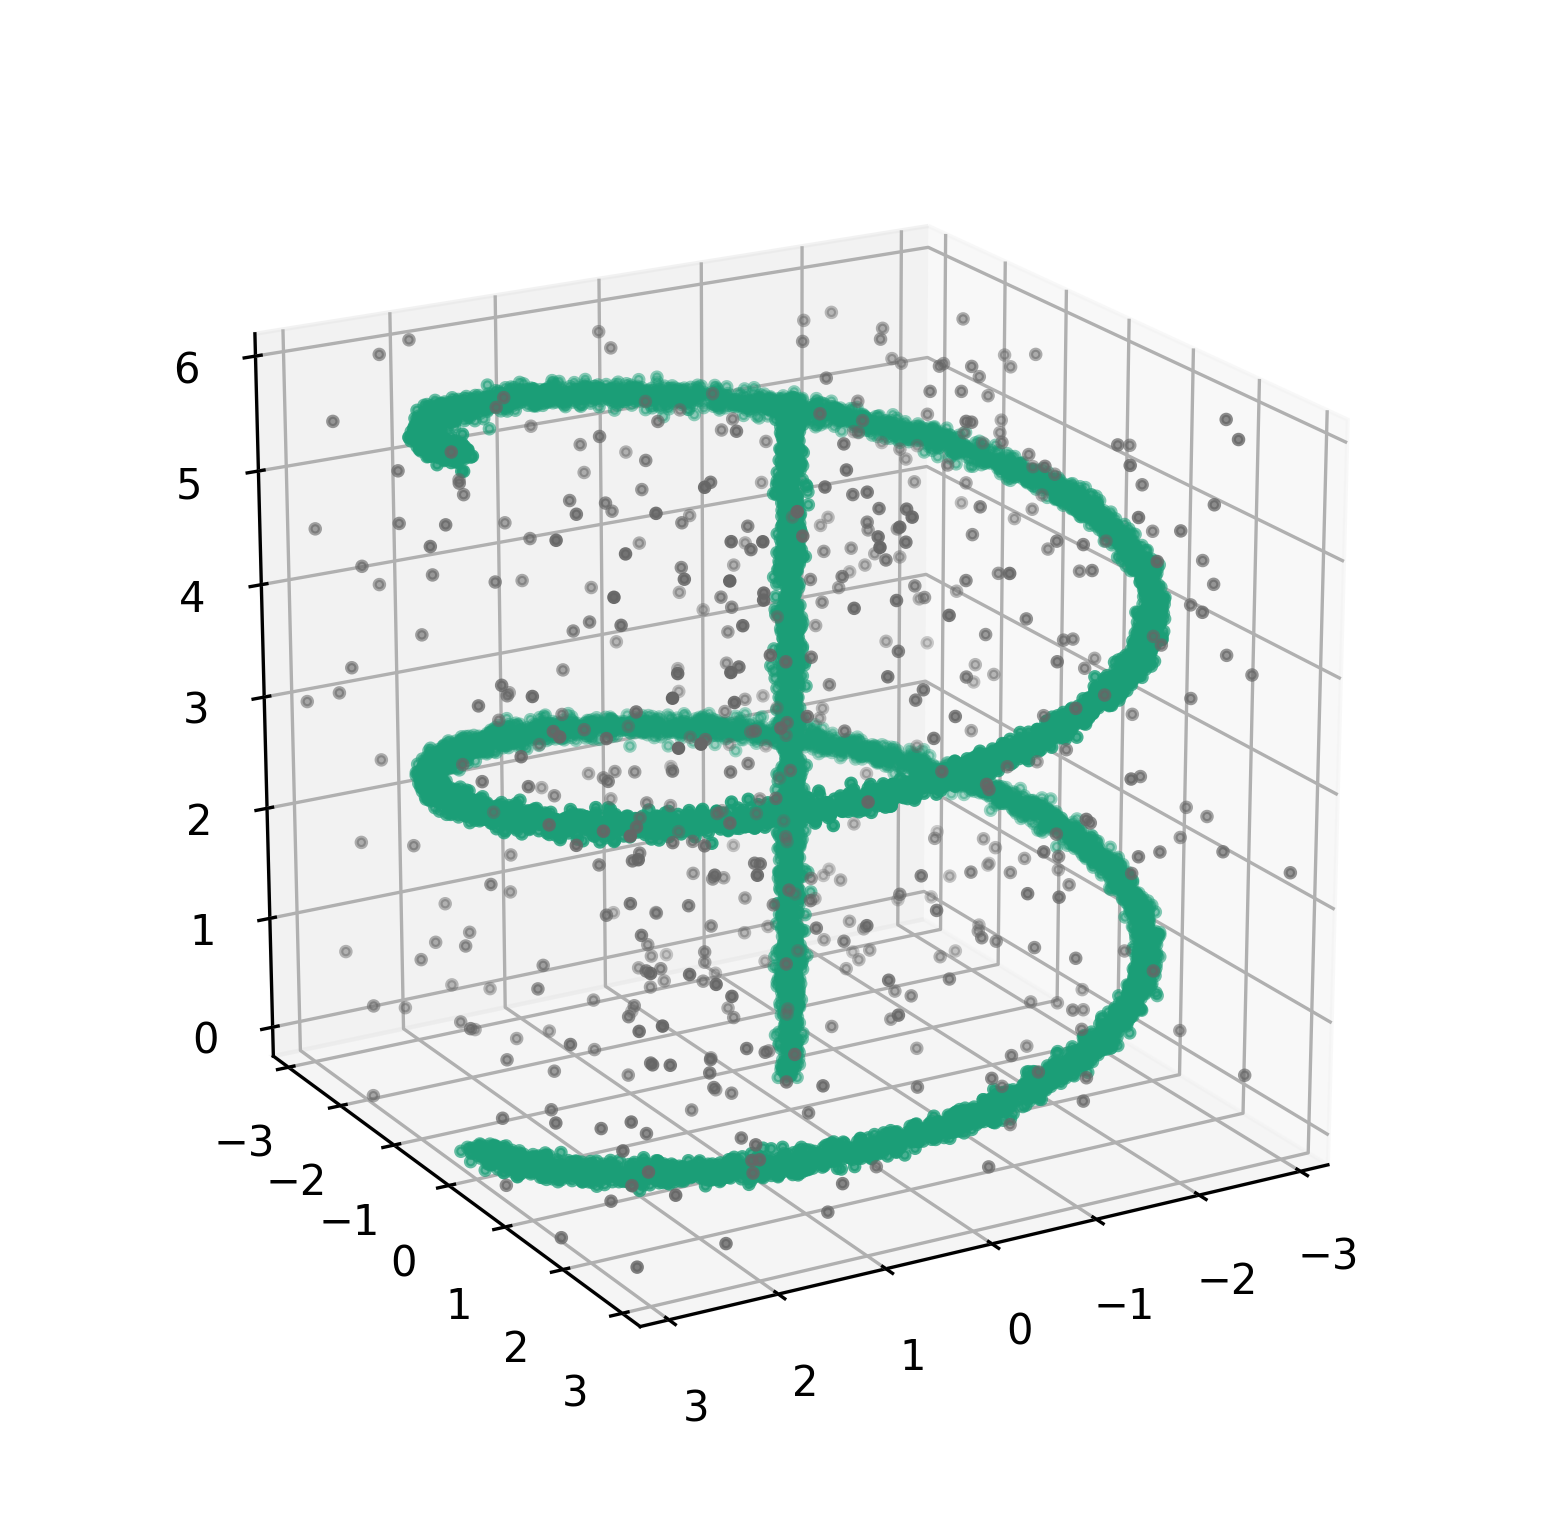
\includegraphics[width=3in]{static/skewer.png}
\caption{The Bullseye (top-left), Spiral (top-right), Interlocking Tori (bottom-left) and Skewer (bottom-left) datasets.}
\label{results:datasets}
\end{figure}

Each dataset was clustered using the l2-distance metric.
We have to be careful to not let the graph shatter and so we used the following stopping criteria for building the cluster tree:

\begin{itemize}
    \item Minimum Cluster Radius: 0.1
    \item Minimum Cluster Cardinality: 1
    \item Maximum Depth: 20
\end{itemize}

We chose to use Min-Max Scaling for normalizing anomalousness measures since it gives us a nice $[0, 1]$ range.
For each dataset, we present the True Positive Rate (TPR), the True Negative Rate (TNR), and a histogram of measured anomalousness.

Table~\ref{results:table} lists the True Positive Rate and the True Negative Rate for each dataset using each of four methods.

Figures~\ref{results:histograms:kth_nearest}, \ref{results:histograms:hierarchical}, \ref{results:histograms:outrank}, and \ref{results:histograms:k_neighborhood} shows histograms of measured anomalousness for points in each dataset for each method used.
Higher values of anomalousness indicate higher confidence that the point is an anomaly.

\begin{table}[!t]
\renewcommand{\arraystretch}{1.3}
\caption{Anomaly Detection performance on the synthetic datasets.}
\label{results:table}
\centering
\begin{tabular}{|c|c|c|c|c|c|c|c|c|}
\hline
 & \multicolumn{2}{c|}{\textbf{Bullseye}} & \multicolumn{2}{c|}{\textbf{Spiral}} & \multicolumn{2}{c|}{\textbf{Interlocking}} & \multicolumn{2}{c|}{\textbf{Skewer}} \\
  & \multicolumn{2}{c|}{\textbf{ }} & \multicolumn{2}{c|}{\textbf{ }} & \multicolumn{2}{c|}{\textbf{Tori}} & \multicolumn{2}{c|}{\textbf{ }} \\
\hline
 & \bfseries TPR & \bfseries TNR & \bfseries TPR & \bfseries TNR & \bfseries TPR & \bfseries TNR & \bfseries TPR & \bfseries TNR \\
\hline
\bfseries k$^{th}$-nearest Distances & 1.000 & 0.979 & 1.000 & 0.020 & 1.000 & 0.979 & 1.000 & 0.979 \\
\hline
\bfseries Hierarchical Sparseness & 0.985 & 0.940 & 1.000 & 0.969 & 0.992 & 0.961 & 1.000 & 0.967 \\
\hline
\bfseries Outrank Algorithm & 0.998 & 0.990 & 1.000 & 0.987 & 1.000 & 0.989 & 1.000 & 0.989 \\
\hline
\bfseries k-Neighborhood Size & 0.996 & 0.990 & 0.990 & 0.984 & 0.761 & 0.986 & 0.975 & 0.983 \\
\hline
\end{tabular}
\end{table}

\begin{figure}[!t]
\centering
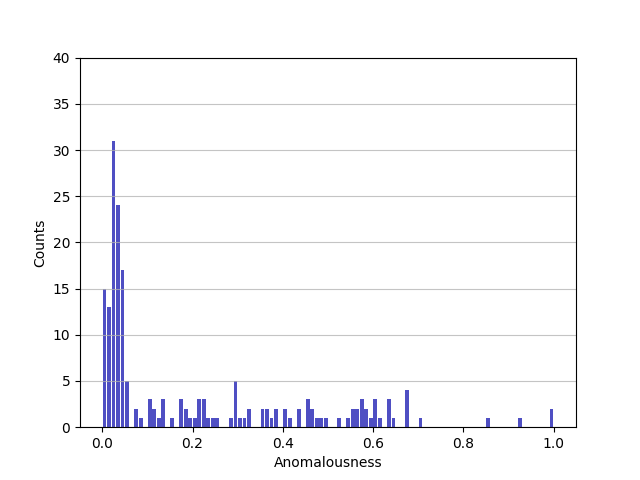
\includegraphics[width=2.5in]{static/bullseye_kth_nearest.png}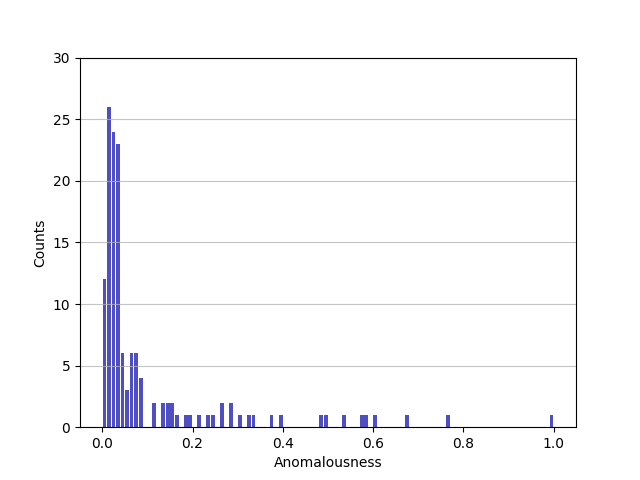
\includegraphics[width=2.5in]{static/spiral_kth_nearest.png}

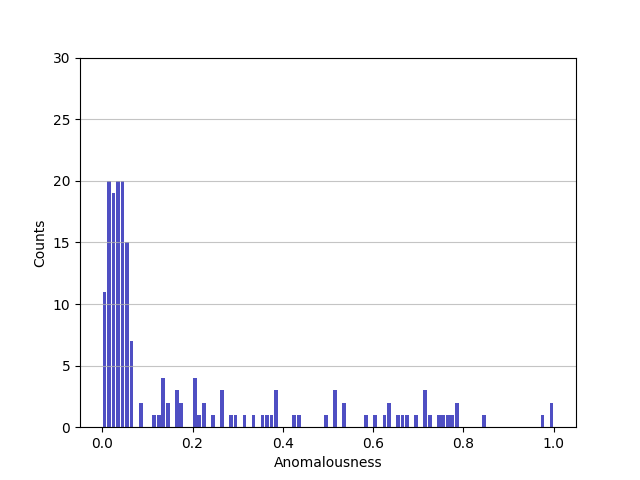
\includegraphics[width=2.5in]{static/interlocking_tori_kth_nearest.png}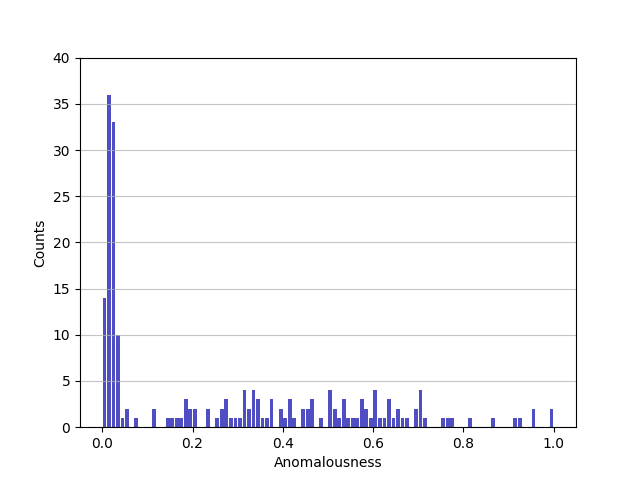
\includegraphics[width=2.5in]{static/skewer_kth_nearest.png}

\caption{
Measures of anomalousness using the k$^{th}$-nearest Distances method on the Bullseye (top-left), Spiral (top-right), Interlocking-Tori (bottom-left), and the Skewer (bottom-right) datasets.
}

\label{results:histograms:kth_nearest}
\end{figure}


\begin{figure}[!t]
\centering
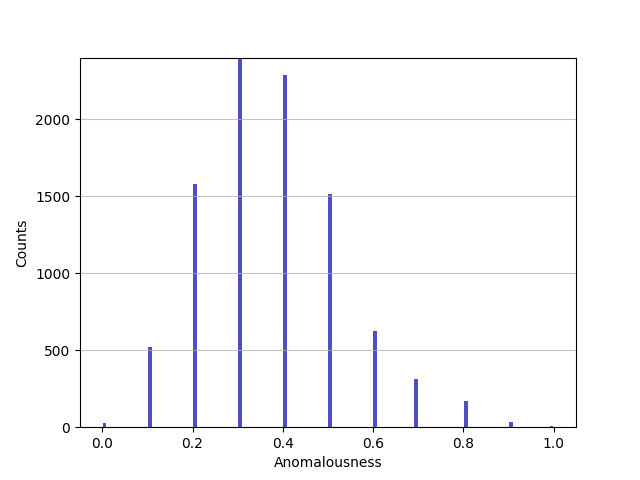
\includegraphics[width=2.5in]{static/bullseye_hierarchical.png}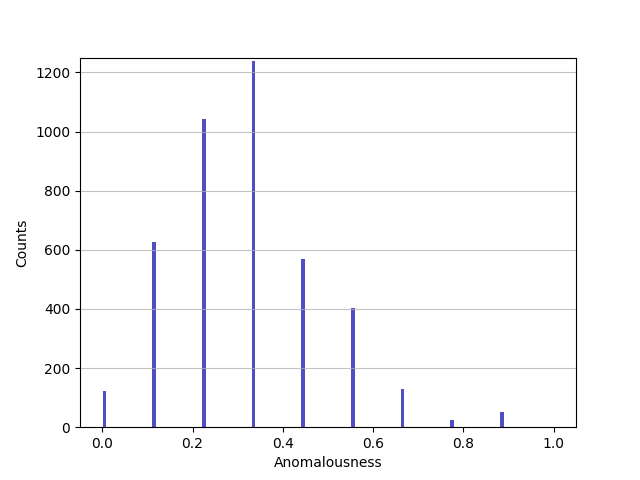
\includegraphics[width=2.5in]{static/spiral_hierarchical.png}

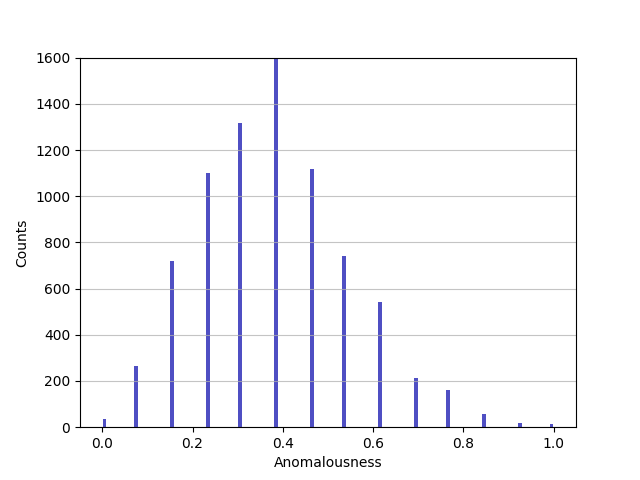
\includegraphics[width=2.5in]{static/interlocking_tori_hierarchical.png}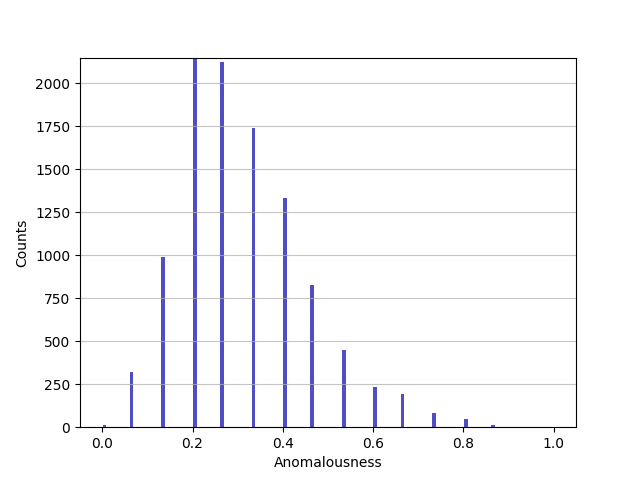
\includegraphics[width=2.5in]{static/skewer_hierarchical.png}

\caption{
Measures of anomalousness using the Hierarchical Sparseness method on the Bullseye (top-left), Spiral (top-right), Interlocking-Tori (bottom-left), and the Skewer (bottom-right) datasets.
}

\label{results:histograms:hierarchical}
\end{figure}


\begin{figure}[!t]
\centering
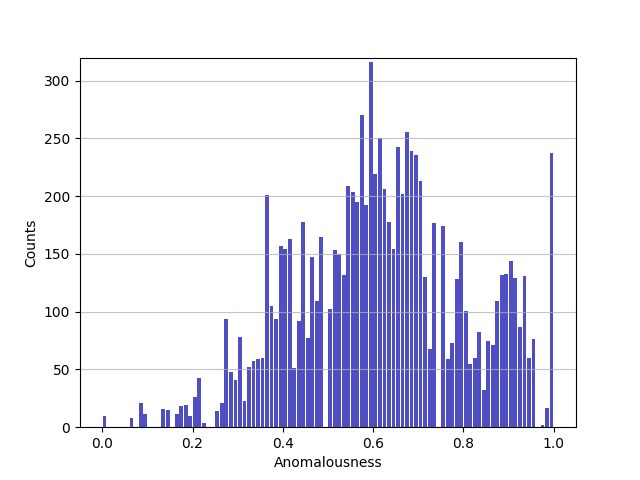
\includegraphics[width=2.5in]{static/bullseye_outrank.png}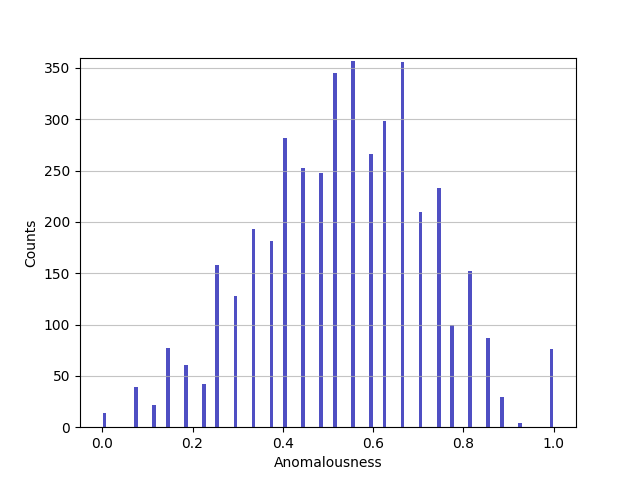
\includegraphics[width=2.5in]{static/spiral_outrank.png}

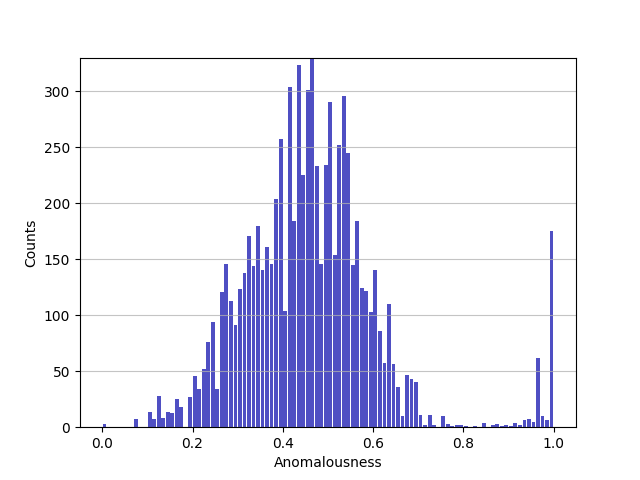
\includegraphics[width=2.5in]{static/interlocking_tori_outrank.png}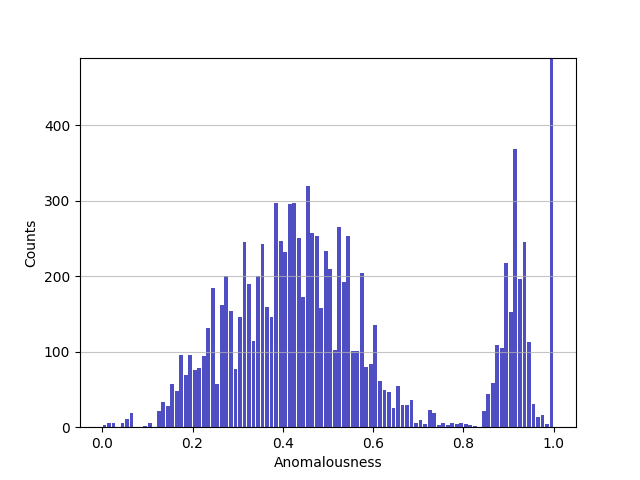
\includegraphics[width=2.5in]{static/skewer_outrank.png}

\caption{
Measures of anomalousness using the Outrank Algorithm on the Bullseye (top-left), Spiral (top-right), Interlocking-Tori (bottom-left), and the Skewer (bottom-right) datasets.
}

\label{results:histograms:outrank}
\end{figure}


\begin{figure}[!t]
\centering
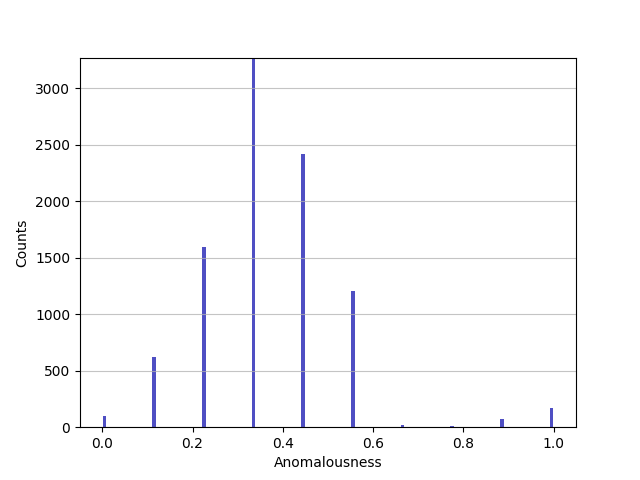
\includegraphics[width=2.5in]{static/bullseye_k_neighborhood.png}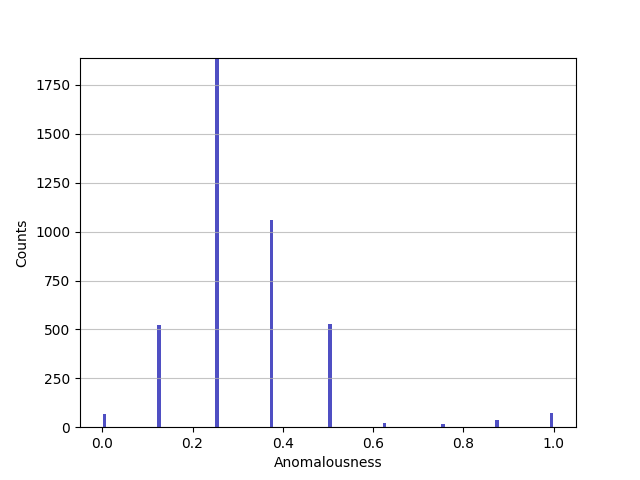
\includegraphics[width=2.5in]{static/spiral_k_neighborhood.png}

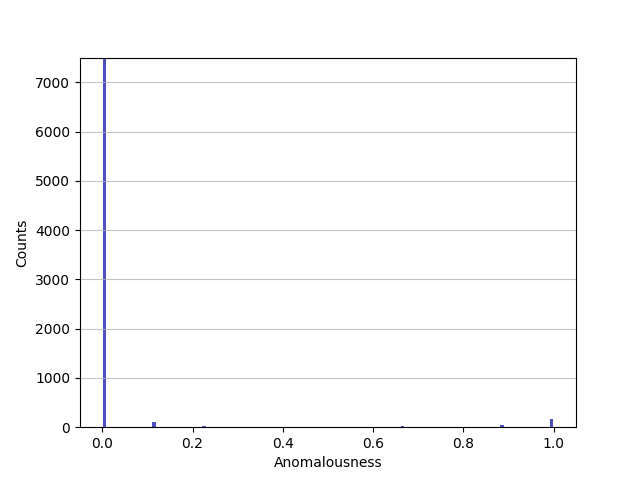
\includegraphics[width=2.5in]{static/interlocking_tori_k_neighborhood.png}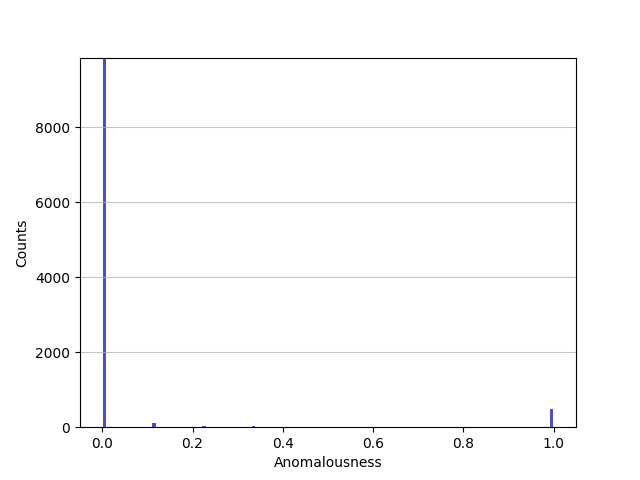
\includegraphics[width=2.5in]{static/skewer_k_neighborhood.png}

\caption{
Measures of anomalousness using the k-Neighborhood Size method on the Bullseye (top-left), Spiral (top-right), Interlocking-Tori (bottom-left), and the Skewer (bottom-right) datasets.
}

\label{results:histograms:k_neighborhood}
\end{figure}
